\subsection{Sensors}

\subsubsection{Landmine Detection Techniques}

Landmine detection technologies have evolved to encompass a wide range of sensing principles, each targeting specific physical, chemical, or biological characteristics of surface-laid and buried mines. Broadly, these methods can be categorized into five general classes: \textit{\textbf{electromagnetic induction-based} techniques}, \textit{\textbf{radiowave and microwave-based} systems}, \textit{\textbf{mechanical and vibro-acoustic} methods}, \textit{\textbf{spectral and thermal imaging} approaches}, and \textit{\textbf{chemical and biological} sensing methods}. Within each class, a variety of specialized detection technologies have been developed, including traditional metal detectors, ground-penetrating radar, infrared and hyperspectral imaging, seismic/acoustic sensors, vapor detection, and biosensors. Each of these approaches offers distinct advantages and faces specific limitations, especially when adapted to drone-based platforms for remote and efficient minefield scanning. In the following subsections, each class is explored in detail, with emphasis on the operating principles, detection capabilities, challenges, and documented UAV-based applications.

\paragraph{Electromagnetic Induction-Based Techniques}

Electromagnetic induction (EMI) methods operate by exploiting the interaction between electromagnetic fields and conductive or magnetic materials in the ground. These systems are typically composed of a transmitter coil that emits a time-varying electromagnetic field into the soil. When this field encounters a conductive object—such as a landmine with metallic components—it induces eddy currents within the object, which in turn generate a secondary magnetic field. This field is detected by a receiver coil, and the resulting signal is processed to infer the presence of the object. These principles form the basis of conventional \textbf{metal detectors}.

In contrast, \textbf{magnetic sensors} or magnetometers do not actively induce eddy currents but instead measure disturbances in the Earth's ambient magnetic field caused by nearby ferromagnetic objects. While metal detectors rely on electromagnetic induction to detect a wide range of conductive materials, magnetometers are primarily sensitive to ferrous (iron-containing) materials and are particularly effective in detecting anomalies in the magnetic environment.

Several specialized EMI sensors have been developed, including induction coil imaging systems that generate spatial maps of subsurface metallic objects, conductivity meters that monitor variations in soil conductivity through eddy current decay, and a range of magnetometers such as fluxgate, proton precession, optically pumped atomic, and meandering winding designs. Each sensor type offers specific trade-offs in sensitivity, resolution, and robustness, and may be selected based on the expected mine characteristics and deployment constraints~\cite{Gooneratne2004ARO, Bruschini1997ASO}.

\textbf{Strengths:} Electromagnetic induction (EMI) methods are among the most mature and widely adopted landmine detection techniques. They are well-established, commercially available, and commonly implemented in handheld and vehicle-mounted systems~\cite{gichd2006guidebook}. These methods are particularly effective for detecting the vast majority of deployed landmines that contain some amount of metal, including minimum-metal mines where metallic elements are limited to components such as detonator capsules or striker pins~\cite{gichd2006guidebook}. With appropriately sized coil systems, EMI devices can achieve considerable depth penetration—for example, up to 70 cm for unexploded ordnance (UXO) and metallic mines~\cite{gichd2006guidebook}. Magnetic sensors, in particular, are versatile and have been applied beyond demining, including the detection of buried utilities, iron ore deposits, archaeological artifacts, and submarines due to their sensitivity to ferrous materials \footnote{\url{https://www.sphengineering.com/integrated-systems/technologies/magnetometer}}.

\textbf{Limitations:} Despite their widespread use, EMI-based methods have significant limitations. A key drawback is their inability to distinguish between landmines and other metallic objects, often leading to very high false alarm rates—ranging from 100 to 1000 false detections per real mine in cluttered environments~\cite{Bruschini1997ASO, robledo2009survey}. Their effectiveness decreases significantly when detecting modern plastic-cased or low-metal-content mines, which often contain only a few grams of metal~\cite{gichd2006guidebook}. These sensors are also susceptible to interference from magnetic or conductive soils, such as laterite-rich ground or coastal sands, and their performance deteriorates in the presence of electromagnetic noise from power lines and nearby electronics~\cite{gichd2006guidebook}. Additionally, footprint size reduces with depth, and passive magnetometers may fail to detect certain non-ferrous materials, such as gold or copper, which do not significantly alter the ambient magnetic field\footnote{\url{https://www.sphengineering.com/integrated-systems/technologies/magnetometer}}.

\textbf{Drone-Based Applications:} EMI sensors have been successfully integrated into unmanned aerial vehicle (UAV) platforms in numerous studies~\cite{yoo2020drone,7529819,mu2020automatic,yoo2021application,BARNAWI2022441,rs15153813,barnawi2023graph,Barnawi2023ADL,s21093175,9251007,Safatly04032021,10745471,Stankevich2024OpticalAM,Joo2022OptimizationDM,rs16162916,Yoo2024UnmannedAV,rs16244732,Poliachenko_Kozak_Bakhmutov_Cherkes_Bilyi_2025}. These include implementations of both lightweight metal detectors and magnetic sensors for aerial surveying of minefields. Figure~\ref{fig:metal_detector_drone} shows an example of a UAV equipped with a metal detector for low-altitude scanning, while Figure~\ref{fig:magnetometer_drone} illustrates a UAV-mounted magnetometer designed for aerial magnetic anomaly detection. 

\begin{figure}[h!]
    \centering
    \begin{subfigure}[b]{0.48\linewidth}
        \centering
        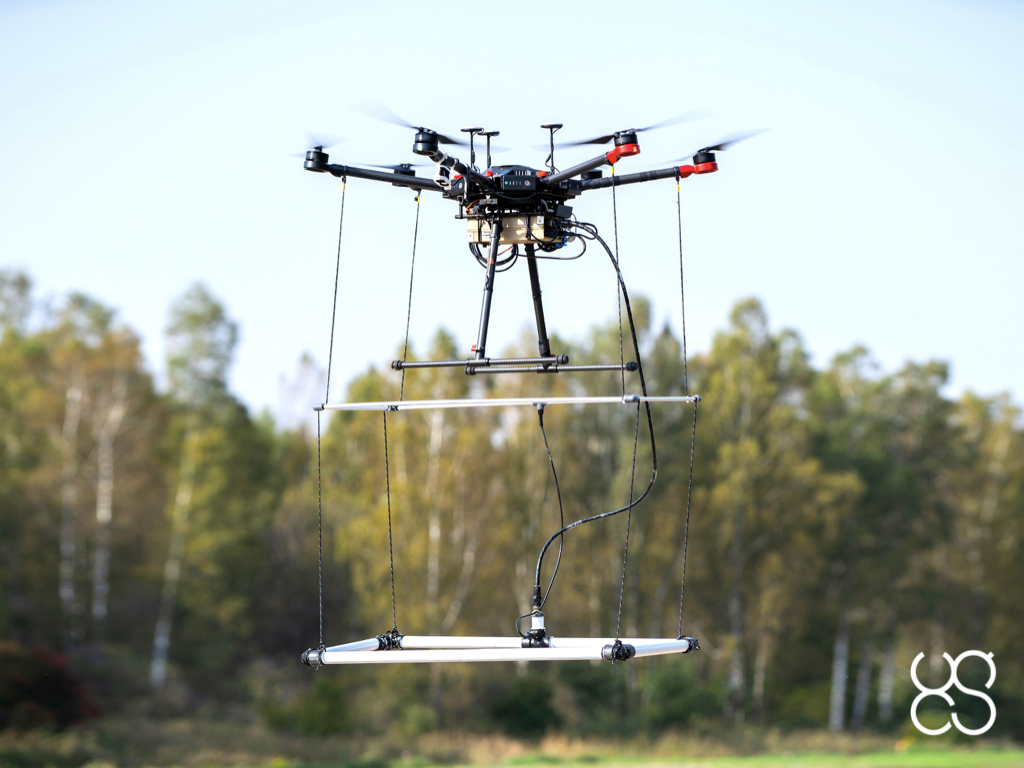
\includegraphics[width=\linewidth]{figs/Huirui/metal_detector_drone.png}
        \caption{UAV-mounted metal detector system\protect\footnotemark.}
        \label{fig:metal_detector_drone}
    \end{subfigure}
    \hfill
    \begin{subfigure}[b]{0.48\linewidth}
        \centering
        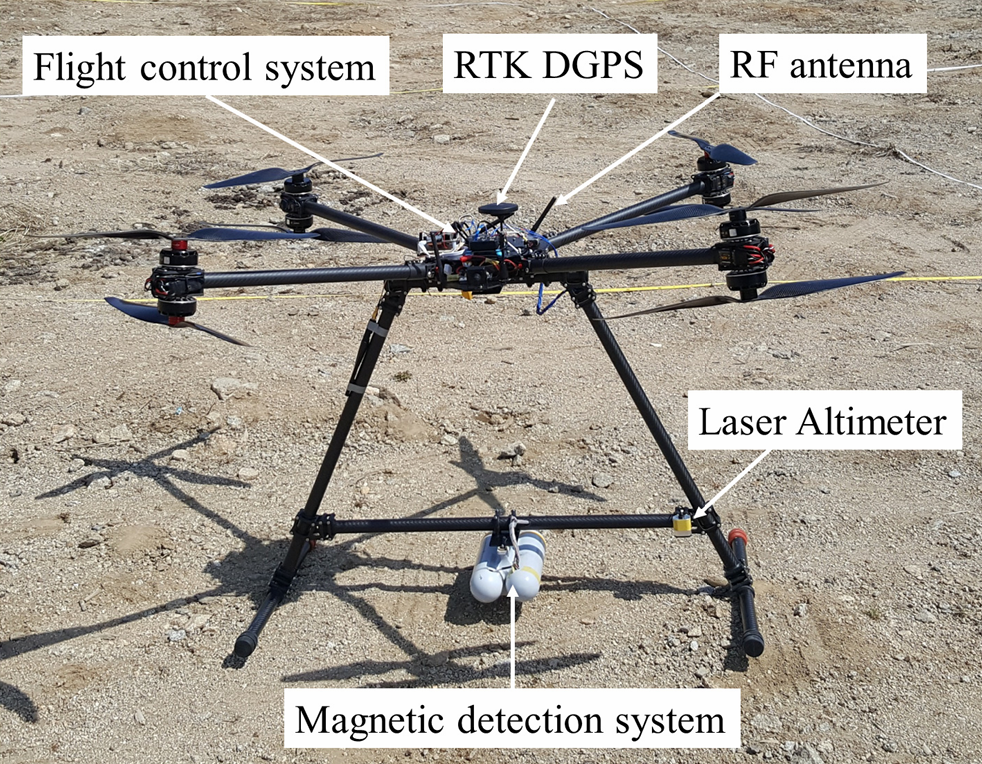
\includegraphics[width=\linewidth]{figs/Huirui/magnetometer_drone.png}
        \caption{Drone-based magnetometer platform~\cite{yoo2020drone}.}
        \label{fig:magnetometer_drone}
    \end{subfigure}
    \caption{Examples of UAV platforms integrating electromagnetic sensors for landmine detection.}
    \label{fig:emi_uav_examples}
\end{figure}

\footnotetext{\url{https://www.sphengineering.com/news/sph-engineering-introduces-the-drone-integrated-metal-detection-system}}
